\section{Die Webseite}
Die Webseite der Wetterstation ist mit dem CMS Openfile64Light der Firma Screenbox erstellt. Der Nachteil am CMS ist, dass auf der Seite selber keine eigenen HTML, CSS oder Javascript Dateien erlaubt. Eigene Änderungen oder dynamische Inhalte, werden in openfile64Light als sogenannte Applikationen behandelt. Um eigene Inhalte zu erstellen muss für die gewünschte Applikation eine PHP Referenzdatei erstellt werden, welche auf die HTML, Javascript und CSS Dateien in einem eigenen Ordner verweisen,diese muss im Ordner application abgelegt werden und in der Datenbank in der Tabelle applications gespeichert werden.\\

Für die Anzeige der von Weather-Display ausgewerteten Daten läuft wird Weather-Display Live. Das Weather-Display live funktioniert mit Flash, dies wird jedoch, aus folgendem Grund, nicht mehr von allen Geräten unterstützt, war jedoch zu beginn des Internetzeitalters essentiell für dynamische Webseiten. Mit ihm konnten einfach dynamische Inhalte erstellt und administriert werden. Jedoch gab es immer wieder gravierende Sicherheitslücken und Weiterentwicklungen im Bereich Web. Mit dem aufkommen der Smartphones wurde Flash immer weiter verdrängt durch HTML5 und Javascript. Nicht zuletzt auch durch ein Kommuniqué von Steve Jobs. In diesem erklärt er warum seine Firma (Apple) nicht auf Flash, sondern HTML5 und Javascript setzt. Einer der Gründe für dieser Entscheidung ist, dass Flash keine open-source Software ist. D.h Adobe kontrolliert das System. Hierbei erwähnt Steve Jobs auch das Apple ein closed-source system ist, sie jedoch an einen offenen Webstandard glauben. Der zweite Grund ist warum Apple sich nicht für Flash entschieden hat ist, dass die Videos bzw. Games seit diesem offenen Brief aus dem Jahr 2009 auch in den neuen Standards, H.264, erhältlich ist. Der dritte Grund, das Apple nicht auf Flash gesetzt hat ist die Sicherheit. Aus Untersuchungen im Jahr 2009 ging hervor, dass die ihre Macs abstürzen. Dies kommt durch die Flashsoftware von Adobe. Dazu kommt, dass Flash auf den mobilen Geräten von Apple nicht sicher lief. Mehrmals wurde Adobe gefragt um eine laufende Version zu erstellen, dies hat Adobe jedoch nicht geschafft. Aus diesen Gründen hat Apple, welcher einer der Vorreiter von Smartphones war, sich entschieden um Flash nicht zu benutzen. Dadurch haben auch andere Hersteller von mobilen Geräten nachgezogen und auf Flash möglichst verzichtet. \cite{Apple:ThoughtsOnFlash} \\
Der wichtigste Grund ist das Adobe ab 2020 Flash nicht mehr weiterentwickelt und keine Updates mehr herausgeben wird. Dies aufgrund der oben genannten Tatsachen und das zur heutigen Zeit vielmals Flash umgangen wird und andere Lösungen gebraucht werden. Aufgrund von dies wird ab 2020 auch kein Browser mehr das Plugin zulassen und Seiten welche Flashinhalte benutzen sind nicht mehr Vollständig verfügbar. Somit ist auch die Wetter-Arbon Seite von dieser Tatsache betroffen. \cite{Adobe:FlashTheFutureofInteractiveContent}\\
Um trotzdem erreichbar, auf Endgeräte ohne Flash, zu sein wird in der Wassersport.php bzw. Touristik.php Datei der Entscheid gefällt ob die Flash-Seite oder die Bild-Seite geöffnet wird, im Code des Wassersport.php-File oder im Touristik.php-File, je nachdem welche Seite geöffnet wird gefällt. Dies wird mit folgendem Code entschieden: 

\begin{lstlisting}
if (swfobject.hasFlashPlayerVersion("1")) {
document.write('
<iframe 
src="https://www.wetter-arbon.ch/WDL/index.html">
</iframe>');
} 
else {
document.write('
<img class="pageImage" 
src="https://www.wetter-arbon.ch/WDL/WDL.png" alt="Bodensee West" 
/>');
}
\end{lstlisting}

Der Nachteil an der Bild-Seite ist jedoch, dass die Anzeigen nicht mehr dynamisch sind. So wird z.B. die Änderung der Windrichtung nicht angepasst und muss stetig von Hand aktualisiert werden, will man den aktuellen Wert sehen.\\

Zusätzlich zur Desktop-Seite, auf welcher alle Informationen verfügbar sind, gibt es eine mobile abgespeckte Version der Wetterstation, siehe \ref{img:mobilewebseite} auf Seite \pageref{img:mobilewebseite}, diese ist erreichbar unter m.wetter-arbon.ch. Auf dieser werden die zwei aktuellsten Bilder der Touristikseite, bzw. der Wassersportseite auf einer Seite dargestellt. Zusätzlich gibt es einen Link welche die Bilder der Webcam, sowie deren Steuerungseinheit darstellt.
\begin{figure}[htbp]
	\centering
	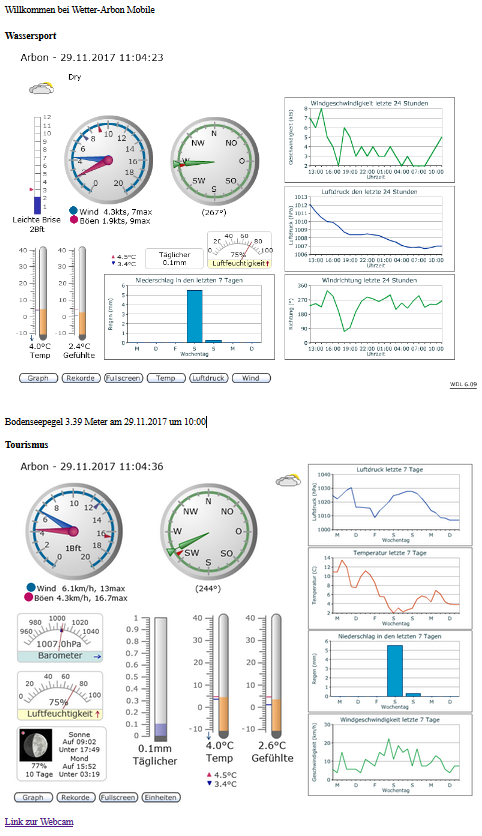
\includegraphics[width=0.9\linewidth]{img/mobile_webseite}
	\caption{Datenanzeige m.wetter-arbon.ch}
	\label{img:mobilewebseite}
\end{figure}

Das Problem der Webseite und vorallem der verschiedenen Applikationen ist, dass viele Geräte Flash nicht mehr oder in naher Zukunft nicht mehr unterstützen. Zusätzlich ist die Lösung mit dem Screenshot der aktuellen Verhältnisse auch keine optimale Lösung. Auch sind die Schreibfehler, welche entdeckt wurden bei näherer Betrachtung auch nicht Vorteilhaft. Weiter ist die Wetterapplikation nicht nach dem Prinzip responsive Design aufgebaut, welches in der heutigen Zeit ein wichtiger Bestandteil einer Webseite ist. Zusätzlich zum Flash, von der Gebrauch gemacht wird sind die Anzeigen auf der Touristik bzw. Wassersport Seite unschön. Die Graphen, bspw. der Windanzeige mit ihrer Richtung sowie die Stärke, sind schwer lesbar, da die Skalierung des Graphen\Diskussionspunkt{Bild zweier Graphen, als Vergleich} automatisch die, je nach Windstärke, wechselt.

\begin{figure}[htbp]
	\centering
	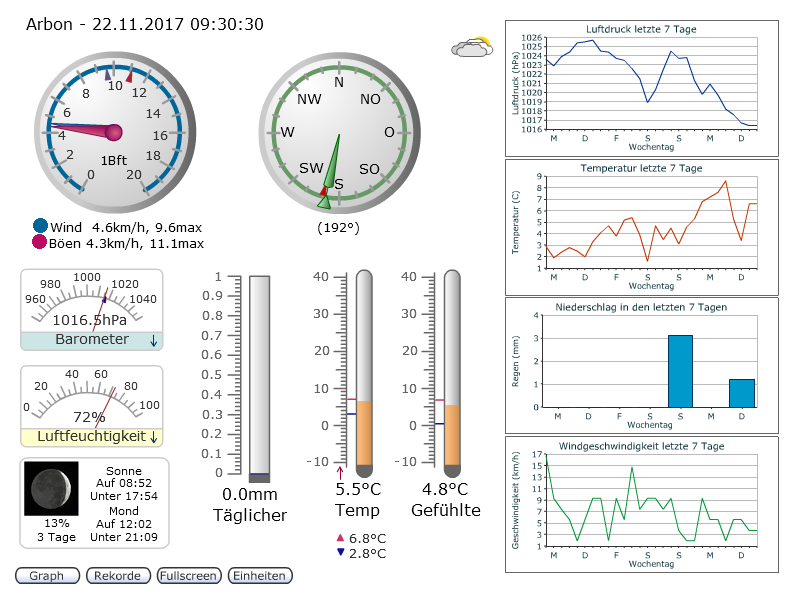
\includegraphics[width=0.9\linewidth]{img/grafik}
	\caption{Datenanzeige wetter-arbon.ch}
	\label{img:grafik-dummy}
\end{figure}

Um die Webseite auf den neusten Stand der Technik zu bringen sollten folgende Änderungen durchgeführt werden.Die Flash-Software wird ausgemustert und die Applikation wird auf HTML5 und Javascript umgestellt. Die Webseite soll zudem im responsive Design entwickelt werden, damit auch auf mobilen Geräten die aktuelle Wetterlage sichtbar ist. Die dynamischen, sowie auch die teilweise statischen Anzeigen, werden wo möglich mithilfe der Javascript Bibliothek D3.js oder Google Charts erstellt, hiermit lassen sich ansehnliche und moderne Grafiken erstellen. Die Grafiken, sollten so gestaltet sein das auch Sehbehinderte Personen erkennen wie das Wetter momentan ist. Das heisst beispielsweise, dass die Farben auch für Farbenblinde unterscheidbar sein sollten oder blinde Personen anhand eines Vorleseprogramms erkennen wie das Wetter ist. Ein weiterer Punkt ist die Auswahl der Einheiten, diese sollen nach dem ersten Besuch gespeichert bleiben beim Client mithilfe von Webstorage.  \\
Damit alle erklärten Vorgänge besser verständlich sind, wurde ein Ablaufdiagramm erstellt mit der heutigen Situation und der zukünftigen erwünschten Situation.
\begin{landscape}
\begin{figure}[htbp]
	\centering
	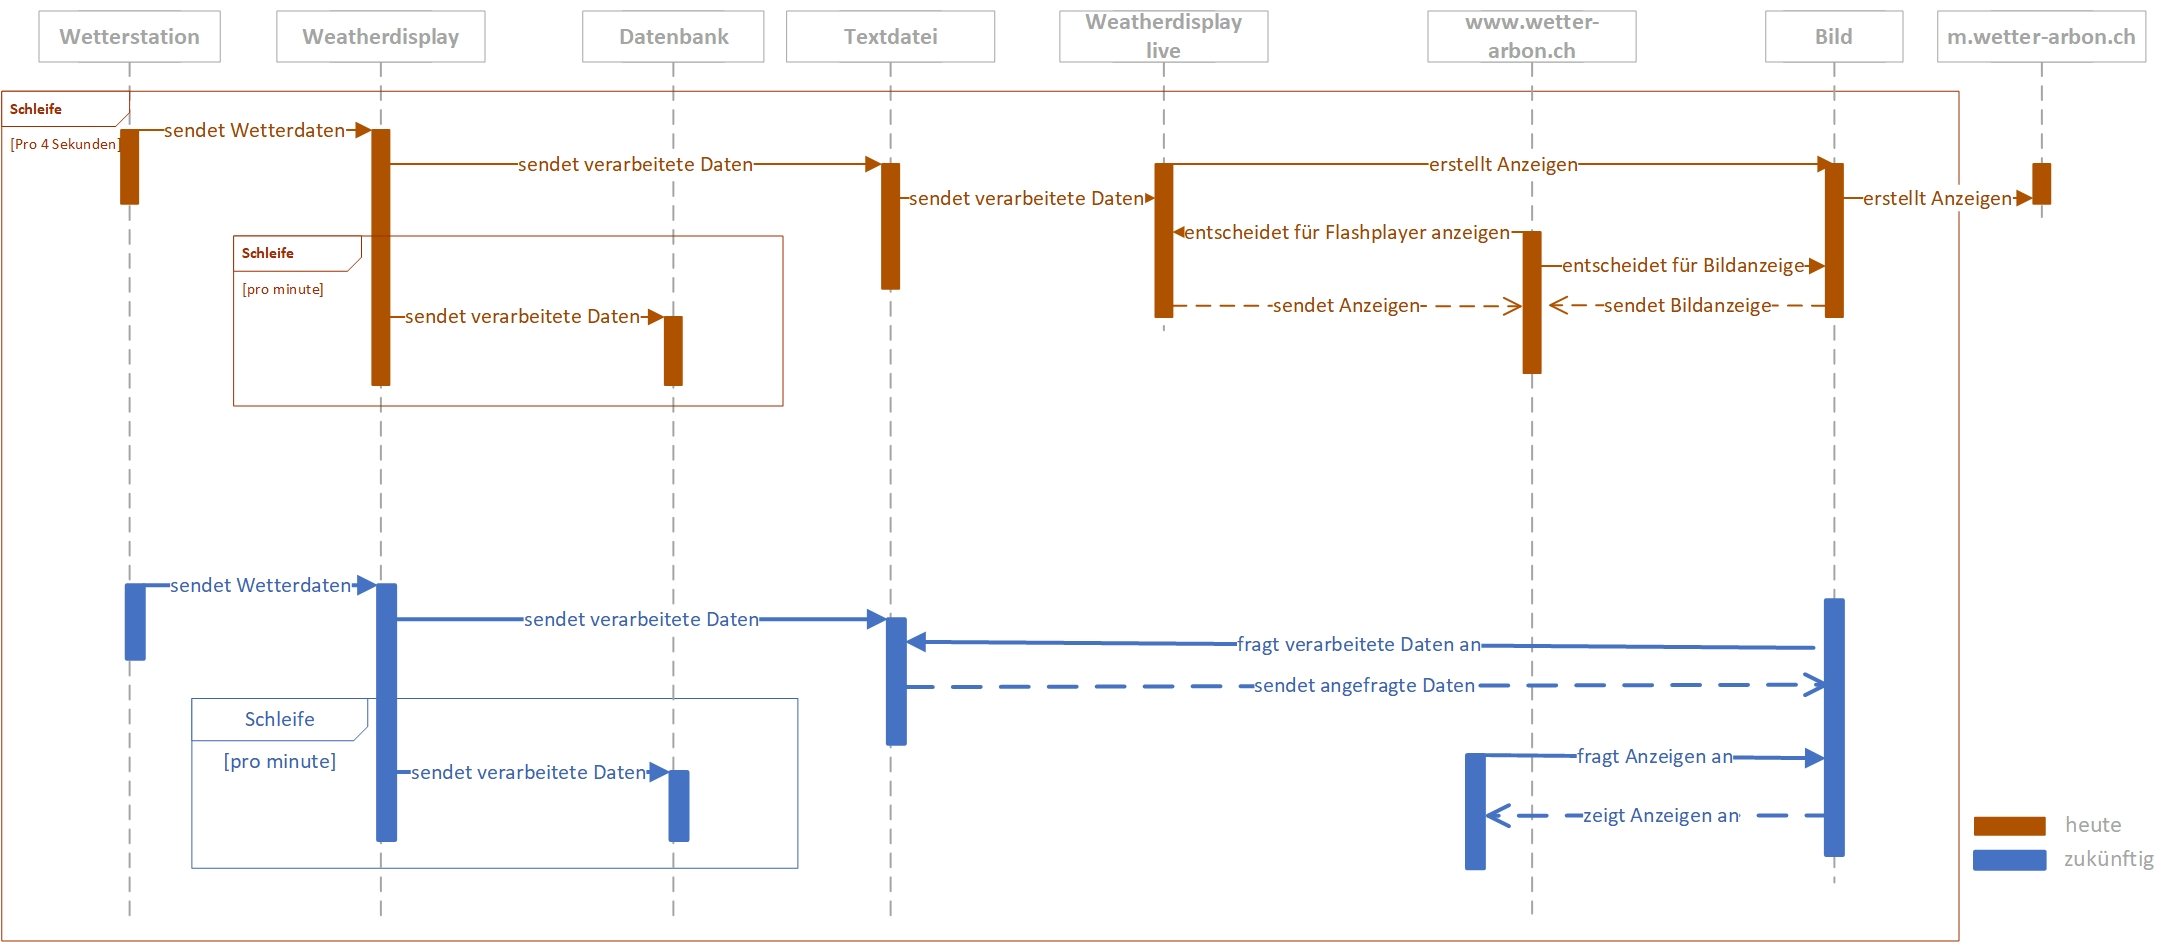
\includegraphics[width=1\linewidth]{img/Sequenzdiagramm_Wetter}
	\caption{Ablauf von der Datenerfassung bis zur Anzeige}
	\label{img:Sequenzdiagramm}
\end{figure}
\end{landscape}